\documentclass[border=5pt]{standalone}
\usepackage{fontspec}
\usepackage{unicode-math}
\setmainfont{Noto Serif}
\newfontfamily\FigureItalic{Noto Serif}
\setmathfont{STIXTwoMath-Regular.otf}
\usepackage{tikz}
\usetikzlibrary{arrows.meta,calc,patterns,decorations.pathmorphing,decorations.markings,decorations.pathreplacing,positioning,backgrounds}
\definecolor{Ink}{HTML}{000000}
\definecolor{Curve}{HTML}{000000}
\definecolor{Bzero}{HTML}{000000}
\definecolor{Bone}{HTML}{000000}
\definecolor{Btwo}{HTML}{000000}
\definecolor{Bthree}{HTML}{000000}
\definecolor{Bfour}{HTML}{000000}
\tikzset{
 ax/.style={draw=Ink,line width=.72pt,-{Latex[length=2.4mm,width=1.5mm]}},
 lev/.style={draw=Ink,line width=1.4pt,line cap=butt},
 thinlev/.style={draw=Ink,line width=.65pt,line cap=butt},
 helper/.style={draw=Ink,line width=.65pt},
 bare/.style={draw=Ink,line width=.95pt,dash pattern=on 4pt off 2.8pt},
 curve/.style={draw=Ink,line width=1.85pt,line cap=round,line join=round},
 ray/.style={draw=Ink,line width=1.0pt,-{Latex[length=2.3mm,width=1.4mm]}},
 measure/.style={draw=Ink,line width=.75pt,{Latex[length=1.9mm,width=1.2mm]}-{Latex[length=1.9mm,width=1.2mm]}},
 link/.style={draw=Ink,line width=1.0pt},
 wave/.style={draw=Ink,line width=.85pt,decorate,decoration={snake,amplitude=.33mm,segment length=2.5mm,pre length=.8mm,post length=.8mm}},
 photon/.style={draw=Ink,line width=1.0pt,-{Latex[length=2.0mm,width=1.3mm]},decorate,decoration={snake,amplitude=.4mm,segment length=2.7mm,pre length=0mm,post length=1.9mm}},
 lab/.style={text=Ink,font=\fontsize{13.5}{16}\selectfont,inner sep=2pt},
 small/.style={text=Ink,font=\fontsize{11.5}{14}\selectfont,inner sep=2pt},
 tag/.style={text=Ink,font=\fontsize{14}{17}\selectfont\FigureItalic\itshape,inner sep=2pt}}
\pagestyle{empty}

\begin{document}
% Figure 12.3; source-grounded revision.
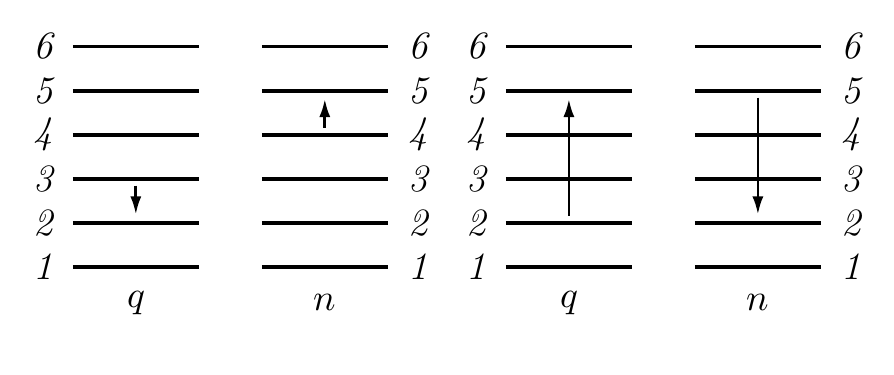
\begin{tikzpicture}[x=1cm,y=1cm]
\coordinate (aQ1) at (0.80000,0.00000);
\coordinate (aQ1L) at (0.00000,0.00000);
\coordinate (aQ1R) at (1.60000,0.00000);
\draw[lev] (aQ1L) -- (aQ1R);
\node[tag,anchor=east] at (-0.18000,0.00000) {1};
\coordinate (aQ2) at (0.80000,0.56000);
\coordinate (aQ2L) at (0.00000,0.56000);
\coordinate (aQ2R) at (1.60000,0.56000);
\draw[lev] (aQ2L) -- (aQ2R);
\node[tag,anchor=east] at (-0.18000,0.56000) {2};
\coordinate (aQ3) at (0.80000,1.12000);
\coordinate (aQ3L) at (0.00000,1.12000);
\coordinate (aQ3R) at (1.60000,1.12000);
\draw[lev] (aQ3L) -- (aQ3R);
\node[tag,anchor=east] at (-0.18000,1.12000) {3};
\coordinate (aQ4) at (0.80000,1.68000);
\coordinate (aQ4L) at (0.00000,1.68000);
\coordinate (aQ4R) at (1.60000,1.68000);
\draw[lev] (aQ4L) -- (aQ4R);
\node[tag,anchor=east] at (-0.18000,1.68000) {4};
\coordinate (aQ5) at (0.80000,2.24000);
\coordinate (aQ5L) at (0.00000,2.24000);
\coordinate (aQ5R) at (1.60000,2.24000);
\draw[lev] (aQ5L) -- (aQ5R);
\node[tag,anchor=east] at (-0.18000,2.24000) {5};
\coordinate (aQ6) at (0.80000,2.80000);
\coordinate (aQ6L) at (0.00000,2.80000);
\coordinate (aQ6R) at (1.60000,2.80000);
\draw[lev] (aQ6L) -- (aQ6R);
\node[tag,anchor=east] at (-0.18000,2.80000) {6};
\node[lab] at (0.80000,-0.45000) {$q$};
\coordinate (aN1) at (3.20000,0.00000);
\coordinate (aN1L) at (2.40000,0.00000);
\coordinate (aN1R) at (4.00000,0.00000);
\draw[lev] (aN1L) -- (aN1R);
\node[tag,anchor=west] at (4.18000,0.00000) {1};
\coordinate (aN2) at (3.20000,0.56000);
\coordinate (aN2L) at (2.40000,0.56000);
\coordinate (aN2R) at (4.00000,0.56000);
\draw[lev] (aN2L) -- (aN2R);
\node[tag,anchor=west] at (4.18000,0.56000) {2};
\coordinate (aN3) at (3.20000,1.12000);
\coordinate (aN3L) at (2.40000,1.12000);
\coordinate (aN3R) at (4.00000,1.12000);
\draw[lev] (aN3L) -- (aN3R);
\node[tag,anchor=west] at (4.18000,1.12000) {3};
\coordinate (aN4) at (3.20000,1.68000);
\coordinate (aN4L) at (2.40000,1.68000);
\coordinate (aN4R) at (4.00000,1.68000);
\draw[lev] (aN4L) -- (aN4R);
\node[tag,anchor=west] at (4.18000,1.68000) {4};
\coordinate (aN5) at (3.20000,2.24000);
\coordinate (aN5L) at (2.40000,2.24000);
\coordinate (aN5R) at (4.00000,2.24000);
\draw[lev] (aN5L) -- (aN5R);
\node[tag,anchor=west] at (4.18000,2.24000) {5};
\coordinate (aN6) at (3.20000,2.80000);
\coordinate (aN6L) at (2.40000,2.80000);
\coordinate (aN6R) at (4.00000,2.80000);
\draw[lev] (aN6L) -- (aN6R);
\node[tag,anchor=west] at (4.18000,2.80000) {6};
\node[lab] at (3.20000,-0.45000) {$n$};
\coordinate (bQ1) at (6.30000,0.00000);
\coordinate (bQ1L) at (5.50000,0.00000);
\coordinate (bQ1R) at (7.10000,0.00000);
\draw[lev] (bQ1L) -- (bQ1R);
\node[tag,anchor=east] at (5.32000,0.00000) {1};
\coordinate (bQ2) at (6.30000,0.56000);
\coordinate (bQ2L) at (5.50000,0.56000);
\coordinate (bQ2R) at (7.10000,0.56000);
\draw[lev] (bQ2L) -- (bQ2R);
\node[tag,anchor=east] at (5.32000,0.56000) {2};
\coordinate (bQ3) at (6.30000,1.12000);
\coordinate (bQ3L) at (5.50000,1.12000);
\coordinate (bQ3R) at (7.10000,1.12000);
\draw[lev] (bQ3L) -- (bQ3R);
\node[tag,anchor=east] at (5.32000,1.12000) {3};
\coordinate (bQ4) at (6.30000,1.68000);
\coordinate (bQ4L) at (5.50000,1.68000);
\coordinate (bQ4R) at (7.10000,1.68000);
\draw[lev] (bQ4L) -- (bQ4R);
\node[tag,anchor=east] at (5.32000,1.68000) {4};
\coordinate (bQ5) at (6.30000,2.24000);
\coordinate (bQ5L) at (5.50000,2.24000);
\coordinate (bQ5R) at (7.10000,2.24000);
\draw[lev] (bQ5L) -- (bQ5R);
\node[tag,anchor=east] at (5.32000,2.24000) {5};
\coordinate (bQ6) at (6.30000,2.80000);
\coordinate (bQ6L) at (5.50000,2.80000);
\coordinate (bQ6R) at (7.10000,2.80000);
\draw[lev] (bQ6L) -- (bQ6R);
\node[tag,anchor=east] at (5.32000,2.80000) {6};
\node[lab] at (6.30000,-0.45000) {$q$};
\coordinate (bN1) at (8.70000,0.00000);
\coordinate (bN1L) at (7.90000,0.00000);
\coordinate (bN1R) at (9.50000,0.00000);
\draw[lev] (bN1L) -- (bN1R);
\node[tag,anchor=west] at (9.68000,0.00000) {1};
\coordinate (bN2) at (8.70000,0.56000);
\coordinate (bN2L) at (7.90000,0.56000);
\coordinate (bN2R) at (9.50000,0.56000);
\draw[lev] (bN2L) -- (bN2R);
\node[tag,anchor=west] at (9.68000,0.56000) {2};
\coordinate (bN3) at (8.70000,1.12000);
\coordinate (bN3L) at (7.90000,1.12000);
\coordinate (bN3R) at (9.50000,1.12000);
\draw[lev] (bN3L) -- (bN3R);
\node[tag,anchor=west] at (9.68000,1.12000) {3};
\coordinate (bN4) at (8.70000,1.68000);
\coordinate (bN4L) at (7.90000,1.68000);
\coordinate (bN4R) at (9.50000,1.68000);
\draw[lev] (bN4L) -- (bN4R);
\node[tag,anchor=west] at (9.68000,1.68000) {4};
\coordinate (bN5) at (8.70000,2.24000);
\coordinate (bN5L) at (7.90000,2.24000);
\coordinate (bN5R) at (9.50000,2.24000);
\draw[lev] (bN5L) -- (bN5R);
\node[tag,anchor=west] at (9.68000,2.24000) {5};
\coordinate (bN6) at (8.70000,2.80000);
\coordinate (bN6L) at (7.90000,2.80000);
\coordinate (bN6R) at (9.50000,2.80000);
\draw[lev] (bN6L) -- (bN6R);
\node[tag,anchor=west] at (9.68000,2.80000) {6};
\node[lab] at (8.70000,-0.45000) {$n$};
\draw[ray,shorten <=2.5pt,shorten >=3pt] (aQ3) -- (aQ2);
\draw[ray,shorten <=2.5pt,shorten >=3pt] (aN4) -- (aN5);
\draw[ray,shorten <=2.5pt,shorten >=3pt] (bQ2) -- (bQ5);
\draw[ray,shorten <=2.5pt,shorten >=3pt] (bN5) -- (bN2);
\node[tag] at (2.00000,-0.95000) {а};
\node[tag] at (7.50000,-0.95000) {б};\end{tikzpicture}

\end{document}
